\documentclass[12pt, titlepage]{article}

\usepackage{booktabs}
\usepackage{comment}
\usepackage{tabularx}
\usepackage{graphicx}
\usepackage{hyperref}
\usepackage{xcolor}
\graphicspath{ {./images/} }
\hypersetup{
    colorlinks,
    citecolor=black,
    filecolor=black,
    linkcolor=red,
    urlcolor=blue
}
\usepackage[round]{natbib}

\title{SE 3XA3: Software Requirements Specification\\Legend of Python}

\author{Team \#1, Lava Boys Inc
        \\ Bilal Jaffry, jaffryb
        \\ Giacomo Loparco, loparcog
        \\ Lucas Zacharewicz, zacharel
}

\date{\today}

\begin{comment}
\input{../Comments}
\end{comment}

\begin{document}

\maketitle

\pagenumbering{roman}
\tableofcontents
\listoftables
{\color{blue}\listoffigures}

\begin{table}[bp]
    \caption{\bf Revision History}
    \begin{tabularx}{\textwidth}{p{3cm}p{2cm}X}
        \toprule {\bf Date} & {\bf Version} & {\bf Notes}\\
        \midrule
        October 5th 2018 & 1.0 & Initial creation\\
        November 8th 2018 & 1.1 & Gave requirements ID's\\
        {\color{blue} December 3rd 2018 & 1.2 & Added Fit Criterion, removed invalid requirements}\\
        \bottomrule
    \end{tabularx}
\end{table}

\newpage

\pagenumbering{arabic}

\section{Project Drivers}

\subsection{The Purpose of the Project}

For many years, Nintendo have been re-releasing NES games for the their other platforms using built in emulators to give the users the same experience of The Legend of Zelda since 1986. With no changes made to the way the game plays in the last 32 years, we aim at modernizing the way The Legend of Zelda will be played by recreating it with new technologies. 

\subsection{The Stakeholders}

\subsubsection{The Customer}

The customer for this project will likely be one who is familiar with The Legend of Zelda series as a whole and would like to experience the original version of the game built upon new technologies. The customer could also be one who has experienced the original game and they would like to compare the two versions.

\subsubsection{The Teaching Assistants and Professor}

The TAs and Professor are directly involved with the project as they are viewing from its start to completion and will being giving guidance on the the various deliveralbes for the project.

\subsubsection{The Developers}

We as the developers are the primary driving force behind the project and will be doing all of the testing, design, aswell as learning new technologies and implementing them into our development for the project.

\subsection{Mandated Constraints}

\begin{itemize}
    \item This program will be able to be run on a computer with  Python3 and the Pygame library
    \item This program will be controlled by the user through their keyboard inputs
    \item This program will output through a display window on the user's monitor
    \item This program will be completed by the assignment-set deadline
\end{itemize}

\subsection{Naming Conventions and Terminology}
\begin{itemize}
    \item The Legend of Zelda: A video game released in the 1980's for the Nintendo Entertainment System (NES), which this project aims to emulate
    \item NES : Nintendo Entertainment System, a video game console released in the 1980's, which ran the original The Legend of Zelda game which this project aims to emulate
    \item AI : Artificial Intelligence, commonly referring to the movement and thought logic of enemies within the game
    \item NPC : Non-playable characters, cannot be controlled by the user. Characters in the game which are only controlled by in-game AI logic.
    \item Nintendo : Video game company, original creators of The Legend of Zelda and the console it is run on
    \item Pygame: Python game engine library in which this project will be built
    \item User: Person operating the game
    \item Player: Playable character within the game
    {\color{blue}\item Sprite: Image used to represent the objects and animation within the game state
    \item Tile: This represents the several accessible rooms in the overarching level}
    \end{itemize}
\newpage
\subsection{Relevant Facts and Assumptions}

It is assumed that the user either has Python3 and Pygame installed in their system, or has internet access to download these necessary tools to run the game, once the repository has been cloned. Also, it is assumed that this game will be run using Python3, as opposed to other Python versions or coding languages.

\section{Functional Requirements}
\subsection{The Scope of the Work and the Product}
{\subsubsection{The Context of the Work}
\begin{figure}[!h]
    \centering
    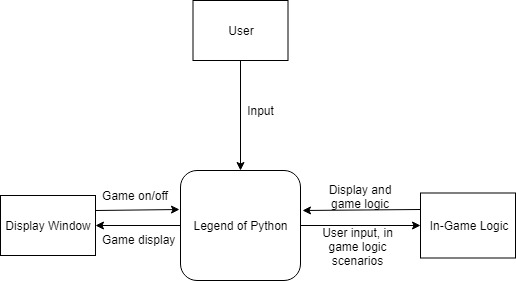
\includegraphics[scale=0.5]{Context.jpg}
    \caption{\color{blue}Context Diagram for The Legend of Python}
    \label{fig:context}
\end{figure}}
\newpage
\subsubsection{Work Partitioning}
    \begin{table}[!h]
        \caption{\bf Game Event List}
        \begin{tabularx}{\textwidth}{p{4cm}p{5cm}X}
            \toprule {\bf Event Name} & {\bf Input and Output} & {\bf Summary}\\
            \midrule
            1 - User runs program & Game On/Off (In), Game Display (Out) & Game start-up, display window created for running Pygame instance\\
            2 - User presses input button & Input (In), User input, in game logic scenarios (Out), Display and game logic(In), Game display(Out) & User movement or menu selection, the input corresponds to a movement or change in the program\\
            3 - User closes program  & Game On/Off (In), Game display (Out) & When the window is closed by the user, the game turns off\\
            \bottomrule
        \end{tabularx}
    \end{table}

\subsubsection{Individual Product Use Cases}

This product has two main use cases, which are operation by the consumer and viewing and editing by a developer. This product, a game, has it's main use case within a user downloading and playing it. This is the main purpose of the program being built. A side use case would be looking at the code, by teaching assistants and professors, and also any developers who come across the project online, and would like to know how it functions and would like to learn and build off of it, similar to what is being done with this project.

\subsection{Functional Requirements}

\begin{enumerate}
    \item Requirement FR1\\ The program must only read inputs from the keyboard connected to the system it is running on\\\\
    {\color{blue}Rationale: To ensure other devices are not obstructing the user in interacting with the game inapporpriately.}
    
    \item Requirement FR2\\The program must only process inputs that would perform an action in the game\\\\
    {\color{blue}Rationale: To only update the game state based on any intended inputs, avoiding undetermined results.}
    
    \item Requirement FR3\\Once the program is running, the program must only take input/output through one display window.\\\\
    {\color{blue}Rationale: To ensure no other external windows/applications are sending inputs to the software when executed.}
    
    \item Requirement FR4\\The program must have a menu on start-up, allowing a user to {\color{blue} start the game by pressing the [K] key}\\\\
    {\color{blue}Rationale: To allow user to choose when to begin the game.}
    
    \item Requirement FR5\\The program must have a pre-defined map, which the player accesses through large tiles (two-dimensional divided sections of the entire map)\\\\
    {\color{blue}Rationale: To ensure the user is bounded by the designed areas of the game.}
    
    \item Requirement FR6\\The program must only allow the player within one tile of the map at a time, and when the end of a tile is reached, the player is transported to the tile next to the current, depending on where the player has exited (if the player leaves the top of the tile, they will be moved to the tile above their current tile)\\\\
    {\color{blue}Rationale: To ensure the player can access different levels of the game in a rationale manner.}
    
    \item Requirement FR7\\The program must have different objects in the map, such as walls which the player and most NPC's cannot pass.\\\\
    {\color{blue}Rationale: To ensure NPC's are unable to access areas of the game, in a way that the game logic is undetermined and to ensure the user does not skip designed areas of the game.}
    
    \item Requirement FR8\\ The program must have items which only the player can collect\\\\
    {\color{blue}Rationale: To allow user to track their progression of the game by collecting player specific items.}
    
    \item Requirement FR9\\ The collectible items should be divided into usable items, collectibles, and consumables\\\\
    {\color{blue}Rationale: To allow user to collect a variety of items.}
    
    \item Requirement FR10\\The program must have items that can be used by the player with input from the user, and ones that cannot be used with input (usable)\\\\
    {\color{blue}Rationale: To allow user to interact with items in a variety of ways.}
    
    \item Requirement FR11\\The program must have an in-game inventory, to allow the user to observe/use their collected items\\\\
    {\color{blue}Rationale: To display to the user their progress throughout the game.}
    
    \item Requirement FR12\\The program must only have one controllable character within the game, with a initial set speed, location, health total and amount, and item inventory\\\\
    {\color{blue}Rationale: To ensure user is only controlling one playable character at a time. This game is intended for single-player use.}
    
    \item Requirement FR13\\The user must be able to control the controllable character with keyboard inputs  once in-game, to move [W,A,S,D] , attack[K], and use an item[L]\\\\
    {\color{blue}Rationale: To allow user to control the player character.}
    
    \item Requirement FR14\\The program must have other non-playable-characters (NPCs) within the game\\\\
    {\color{blue}Rationale: To allow variety of characters for user to encounter while exploring the game}
    
    \item Requirement FR15\\The program must have enemy NPCs, which move and attack with pre-defined logic by the game\\\\
    {\color{blue}Rationale: To allow user to interact with other entities in the game.}
    
    \item Requirement FR16\\The program must have different enemy "classes", with different health amounts, movement speeds, attacks and attack damage values\\\\
    {\color{blue}Rationale: To allow variety for the user when exploring the game.}
    
    \item Requirement FR17\\When the player collides with an enemy NPC, or an enemy NPC attacks the player, the player takes damage, and their health amount is reduced by a values within the range of from 0.5 - 2 hearts\\\\
    {\color{blue}Rationale: To allow feedback for the user when interacting with NPC's, ensuring the NPC attacks are registered on the player character.}
    
    \item Requirement FR18\\When the player attacks an NPC, the NPC's health is reduced by a set value\\\\
    {\color{blue}Rationale: To allow feedback for the user that the attack input has been registered and has changed the state of NPC character.}
    
    \item Requirement FR19\\When the health amount of a character (NPC or player) is reduced to 0, the entity is deemed "dead"\\\\
    {\color{blue}Rationale: To ensure the user and NPC are not invincible and can defeat enemies and be defeated, as is documented in the original game.}
    
    \item Requirement FR20\\When an NPC is dead, it is removed from the current room, and has a chance to drop a heart object or an in-game currenct object. The chance of this drop is randomly generated for each NPC.\\\\
    {\color{blue}Rationale: To reward the user for defeating an enemy.}
    
    \item Requirement FR21\\The program must have 3 consumable items: hearts, an in-game currency and keys\\\\
    {\color{blue}Rationale: To add variety to exploration, provide an reward system for the player accomplishing tasks of defeating enemies and exploring the game.}
    
    \item Requirement FR22\\ The health item must regain health by a value of one at a time, updating the player health to a maximum health of 3.\\\\
    {\color{blue}Rationale: To allow user to continue playing the game even after taking damage from enemy characters.}
    
    \item Requirement FR23\\When the player collides with a  heart/in-game currency consumable object, it is immediately used on the player\\\\
    {\color{blue}Rationale: To allow user to use items while the player is moving, not breaking immersion from the game. }
    
    \item Requirement FR24\\The player must be able to open a locked door if the player collides with the door and they have minimum 1 key. This action will consume a key and bring the player's key count down by one key\\\\
    {\color{blue}Rationale: To ensure user cannot reach an area of the game without exploring certain portions of the game.}
    
    \item Requirement FR25\\When the player is dead, the game is over, and the user is given the options to return to the main menu, or quit the game using the [K] and [Q] keys respectively.\\\\
    {\color{blue}Rationale: To allow user option to continue the game from the beginning after reaching the death screen or to quit the game indefinitely. }
    \item Requirement FR26\\The program must have an objective to follow, getting certain collectible items, and once all set items are collected, the game is completed\\\\
    {\color{blue}Rationale: To give user reason to continue playing the game and to eventually complete the entire game. }
    
    \item Requirement FR27\\The program must have in-game shops, special rooms within the map where the player can buy items with their in-game currency collected over the span of the game\\\\
    {\color{blue}Rationale: To allow user to use their collected items to continue progressing throughout the game.}
\end{enumerate}

\section{Non-functional Requirements}

\subsection{Look and Feel Requirements}
\begin{enumerate}
{\color{blue}\item Requirement NFR1}\\
{\color{blue} Description:} The recreation for The Legend of Zelda should be able to reproduce the similar encounters for the user-controlled character, corresponding to the NES original. The animations for movement and attack should animate the same each time an input is sent by player. 

 {\color{blue}Rationale: This will be used as a way to determine if the game plays similarly to the originally.}\\
 
 {\color{blue}Originator: Giacomo Loparco}\\
 
  {\color{blue}Fit Criterion: The animation sprites for player character changes for every 12 units traveled in the x and y directions for movement, the attack sprite for the player should last for 20 frames. The NPC enemy should be halt its animation if hit by a special usable item.}\\
  
  {\color{blue}Priority: High}
  
  {\color{blue}History: \today}

\subsection{Usability and Humanity Requirements}
{\color{blue}\item Requirement NFR2}\\
{\color{blue} Description:} The software must be simple enough for a user who has played few games, is able to operate it effectively and use all features implemented. The original game was designed for all ages and this recreation must ensure the same accessibility.
{\color{blue}Rationale: This will be used to determine if the game is playable for people with different experiences with gaming}\\

{\color{blue}Originator: Bilal Jaffry}\\

{\color{blue}Fit Criterion: Majority of users who attempt to use the program are able to play the game successfully}\\

{\color{blue}Priority: High}

{\color{blue}History: \today}
\subsection{Performance Requirements}

Speed Requirements

{\color{blue}\item Requirment NFR3} \\
{\color{blue} Description:} The during all gameplay scenarios the game must be able to display the pre-determined refresh rate of 60 Hz and contain a minimum resolution of {\color{blue}480x376 pixels}

{\color{blue}Rationale: This will be used to determine if the games performance in updating the data is consistent and stable.}\\

{\color{blue}Originator: Lucas Zacharewicz, Bilal Jaffry, Giacomo Loparco}\\


{\color{blue}Fit Criterion: This will be measured by an internal frame counter in Pygame does not drop below the 60Hz refresh rate. The display window parameters are created using window constants, ensuring  the ouput window is never smaller/larger than {\color{blue}480x376 pixels} }\\
 
{\color{blue}Priority: High}
  
{\color{blue}History: \today}
  


{\color{blue}\item Requirement NFR4}\\
{\color{blue} Description:} Loading times of each room in a level should be the same for every single segment, properly loading all assets in the same grid position at the same time.

{\color{blue}Rationale: This is will allow for consistent movement between tiles in the game.}\\

{\color{blue}Originator: Lucas Zacharewicz, Bilal Jaffry, Giacomo Loparco}\\

{\color{blue}Fit Criterion: The transition should be done within 2 seconds of loading the next room. The positions of placed objects will be tested to be in same x and y location every time transitioning to different tile.}\\
 
{\color{blue}Priority: High}
  
{\color{blue}History: \today}

Precision Requirements

{\color{blue}\item Requirement NFR5}\\
{\color{blue} Description:} Sprites must render on screen without unforeseen rendering issues

{\color{blue}Rationale: This is ensure the display of the sprites doesn't foresee any weird visual glitches when animating. }\\

{\color{blue}Originator: Lucas Zacharewicz, Bilal Jaffry, Giacomo Loparco}\\

{\color{blue}Fit Criterion: Each tile will be loaded and will be observed for any weird sprite complications from player character or NPC's.}\\
 
{\color{blue}Priority: Medium}
  
{\color{blue}History: \today}

{\color{blue}\item Requirement NFR6}\\
{\color{blue} Description:} All valid player input should respond appropriately for user input through a standard keyboard

{\color{blue}Rationale: This is to ensure the user can only control the player character using any standard keyboard. }\\

{\color{blue}Originator: Lucas Zacharewicz, Bilal Jaffry, Giacomo Loparco}\\

{\color{blue}Fit Criterion: The game will be executed on several systems and keyboard inputs will be checked for consistent for each system.}\\
 
{\color{blue}Priority: Medium}
  
{\color{blue}History: \today}\\
\newpage
Reliability and Availability Requirements

{\color{blue}\item Requirement NFR7}\\
{\color{blue} Description:} The software should continue responding to user input as long as the system is running properly.

{\color{blue}Rationale: This is to ensure Pygame instance can be used/remain idol for long periods of time.}\\

{\color{blue}Originator: Lucas Zacharewicz, Bilal Jaffry, Giacomo Loparco}\\

{\color{blue}Fit Criterion: The game will be run on various systems with other applications running for 180 minutes and will be seen if the game continues to function as intended at every 10 minute interval of the allotted interval. }\\
 
{\color{blue}Priority: Low}
  
{\color{blue}History: \today}

{\color{blue}\item Requirement NFR8}\\
{\color{blue} Description:} There must be no restrictions in obtaining the most recent version of the software

{\color{blue}Rationale: This is to ensure the game is accessible at all times.}\\

{\color{blue}Originator: Bilal Jaffry}\\

{\color{blue}Fit Criterion: The repository should be available to the public as long as GitHub usually maintains public directories. }\\
 
{\color{blue}Priority: Low}
  
{\color{blue}History: \today}
\newpage
Capacity Requirements

{\color{blue}\item Requirement NFR9}\\
{\color{blue} Description:} A user must not need more than 500MB to download and run this software properly

{\color{blue}Rationale: This is to ensure the software is too large for users}\\

{\color{blue}Originator: Bilal Jaffry}\\

{\color{blue}Fit Criterion: The final repository size. including sound and sprite assets will be checked for size under 500MB when the project is completed. }\\
 
{\color{blue}Priority: Low}
  
{\color{blue}History: \today}

\subsection{Operational and Environmental Requirements}
Expected Technological Environment 

{\color{blue}\item Requirement NFR10}\\
{\color{blue} Description:} The user must be able to use any keyboard device as an input device, with the [W,A,S,D] keys being the default method of moving the playable character

{\color{blue}Rationale: This is to ensure the user can only control the player characters movement with only these keys.}\\

{\color{blue}Originator:  Lucas Zacharewicz, Bilal Jaffry, Giacomo Loparco}\\

{\color{blue}Fit Criterion: The game will be run on various systems and the response for movement from [W,A,S,D] keys will be observed.}\\
 
{\color{blue}Priority: High}
  
{\color{blue}History: \today}

{\color{blue}\item Requirement NFR11}\\
{\color{blue} Description:} System specifications must be able to display a minimum resolution of 480x376 pixels, at a 60Hz refresh rate\\
{\color{blue}Rationale: This is to ensure the user attempting to play the game can play it at the minimum specifications.}\\

{\color{blue}Originator:  Lucas Zacharewicz, Bilal Jaffry, Giacomo Loparco}\\

{\color{blue}Fit Criterion: The Pygame instance checks the display device for each system to ensure the set refresh rate and resolution is at the minimum specification.}\\
 
{\color{blue}Priority: Medium}
  
{\color{blue}History: \today}\\

Partner Applications

{\color{blue}\item Requirement NFR12}\\
{\color{blue} Description:} The software must not restrict the use of other processes on the desktop environment running at that given time

{\color{blue}Rationale: This is to ensure when a user decides to use the software it does not interfere with other processes the user wishes to use.}\\

{\color{blue}Originator:  Lucas Zacharewicz, Bilal Jaffry, Giacomo Loparco}\\

{\color{blue}Fit Criterion: The game will be ran on several systems and will be observed during }\\
 
{\color{blue}Priority: Medium}
  
{\color{blue}History: \today}

\newpage
\subsection{Maintainability and Support Requirements}
Maintainability
{\color{blue}\item Requirement NFR13}\\
{\color{blue}Description: } Software revisions should be able to integrate with previous versions without any issues.

{\color{blue}Rationale: This is to ensure that when a user can continue to use the software after an update has been pushes to the repository.}\\

{\color{blue}Originator:  Lucas Zacharewicz, Bilal Jaffry, Giacomo Loparco}\\

{\color{blue}Fit Criterion: Updates will be tested on several systems to monitor functionality of the software after any software revisions have been made. }\\
 
{\color{blue}Priority: Medium}
  
{\color{blue}History: \today}

{\color{blue}\item Requirement NFR14} \\
{\color{blue}Description:} The software should be updated when the software is no longer properly functioning on newer builds of OS environments

{\color{blue}Rationale: This is to ensure that the software application can execute properly when there are updates made on the designated operating systems }\\

{\color{blue}Originator: Bilal Jaffry}\\

{\color{blue}Fit Criterion: The software will be tested for functionality after a mandatory update is made to the designated operating systems. }\\
 
{\color{blue}Priority: Medium}
  
{\color{blue}History: \today}

{\color{blue}\item Requirement NFR15} \\
{\color{blue}Description: } The source code is to be made available for modification and maintainability by anyone

{\color{blue}Rationale: This is to ensure that the software continues to function and maintains its open-source property by being modified and maintained by any user.}\\

{\color{blue}Originator:  Lucas Zacharewicz, Bilal Jaffry, Giacomo Loparco}\\

{\color{blue}Fit Criterion: Users will clone the software repository and alter it. The functionality will be tested after these changes are made.}\\
 
{\color{blue}Priority: Medium}
  
{\color{blue}History: \today}

{\color{blue}\item Requirement NFR16} \\
{\color{blue} Description:} Anyone should be able to find the software and freely download and install the software on the current version of Windows/Linux/{\color{blue}Mac OS}

{\color{blue}Rationale: This is to ensure the software can run on the designated operating systems as intended.}\\

{\color{blue}Originator:  Lucas Zacharewicz, Bilal Jaffry, Giacomo Loparco}\\

{\color{blue}Fit Criterion: The software application will be installed on each designated operating systems and tested for its functionality for booting up, playing and exiting the game.}\\
 
{\color{blue}Priority: High}
  
{\color{blue}History: \today}
\newpage
\subsection{Security Requirements}

{\color{blue}\item Requirements NFR17}\\
{\color{blue} Description: } The source code must be made available for all members of the public to easily access and modify the software

{\color{blue}Rationale: This is to ensure the software maintains its property of being an open-source application, allowing for modification and easy access.}\\

{\color{blue}Originator:  Lucas Zacharewicz, Bilal Jaffry, Giacomo Loparco}\\

{\color{blue}Fit Criterion: The repository will be cloned onto several machines after succesfully searching for the "The Legend of Python" on GitHub.}\\
 
{\color{blue}Priority: Medium}
  
{\color{blue}History: \today}

\subsection{Cultural Requirements}

{\color{blue}\item Requirement NFR18}\\
{\color{blue}Description: } The software will not use any texts, images or media that can potentially offend people from other countries that download and use the software

{\color{blue}Rationale: This is to ensure the software is accessible to anyone and does not intend to harm and offend any persons faith and culture.}\\

{\color{blue}Originator: Bilal Jaffry}\\

{\color{blue}Fit Criterion: The software application will analyzed for any potential discrepancies and will be altered on such discovery. }\\
 
{\color{blue}Priority: Low}
  
{\color{blue}History: \today}

{\color{blue}\item Requirement NFR19}\\
{\color{blue}Description: } The software should give warning to clarify any similarities to any cultural, historical, political figures/event/beliefs are purely coincidental

{\color{blue}Rationale: This is to ensure the software that any remaining similarities in the game are not intended harm and offend any persons faith, culture and political beliefs.}\\

{\color{blue}Originator:  Lucas Zacharewicz, Bilal Jaffry, Giacomo Loparco}\\

{\color{blue}Fit Criterion: The user guide will have a section regarding the potential similarities to any historical, political figures/event/beliefs are and state that they are purely coincidental}\\
 
{\color{blue}Priority: Low}
  
{\color{blue}History: \today}

\subsection{Legal Requirements}
{\color{blue}\item Requirement NFR20}\\
{\color{blue}Description:} The software must not be sold for any monetary gain and must be available freely world wide

{\color{blue}Rationale: This software application is an open-source project, and by definition should be available freely.}\\

{\color{blue}Originator:  Lucas Zacharewicz, Bilal Jaffry, Giacomo Loparco}\\

{\color{blue}Fit Criterion: The GitHub repository is accessible to anyone with access to the site and can be freely cloned and modified.}\\
 
{\color{blue}Priority: Low}
  
{\color{blue}History: \today}

{\color{blue}\item Requirement NFR21}\\
{\color{blue}Description:} The software must agree to following all regulations for the legal distribution of free open source software

{\color{blue}Rationale: This is to ensure the software is following all legal guidelines for the distribution of open-source software.}\\

{\color{blue}Originator:  Lucas Zacharewicz, Bilal Jaffry, Giacomo Loparco}\\

{\color{blue}Fit Criterion: The software follows distribution of permissive free software license using the MIT License framework,}\\
 
{\color{blue}Priority: Low}
  
{\color{blue}History: \today}

\subsection{Health and Safety Requirements}

{\color{blue}\item  Requirement NFR22}\\
{\color{blue}Description:} Frequent breaks of 15 minutes or more should be taken between play sessions lasting longer than 60 minutes

{\color{blue}Rationale: This is to ensure the user doesn't suffer from any fatigue from playing the game and maintains proper health.}\\

{\color{blue}Originator:  Lucas Zacharewicz, Bilal Jaffry, Giacomo Loparco}\\

{\color{blue}Fit Criterion: The user guide for the application will indicate to the user to take breaks after a 60 minute interval of playing the game.}\\
 
{\color{blue}Priority: Low}
  
{\color{blue}History: \today}

{\color{blue}\item Requirement NFR23}\\
{\color{blue}Description: } The software should not compromise the rest of the user’s system before, during and after run-time of the software

{\color{blue}Rationale: This is to ensure the users internal system is not compromsied during the execution and use of the software files.}\\

{\color{blue}Originator:  Lucas Zacharewicz, Bilal Jaffry, Giacomo Loparco}\\

{\color{blue}Fit Criterion: The software is a stand-alone software and only relies on Python libraries for functionality. It does not require any connections to the internet and once cloned the software only has a direct connection to the GitHub repository.}\\
 
{\color{blue}Priority: Low}
  
{\color{blue}History: \today}

\end{enumerate}

\section{Project Issues}

\subsection{Open Issues}

\begin{itemize}
    \item The decision on how the screens are going to be rendered have yet to be made, the current two avenues of thought are loading the whole map and moving the camera around, or only rendering one screen at a time and having room transitions.
    \item The decision to allow for diagonal movement has been pondered as it is a feature in most topdown 2d games these days, but it doesn't blend well with the way movement is already set up in the original game.
\end{itemize}

\subsection{Off-the-Shelf Solutions} 

There are several off the shelf solutions already available to consumers. Nintendo has re-released The Legend of Zelda multiple times across multiple platforms, with the most recent version being released as recently as September 2018 as part of the Nintendo Switch online service. These releases are available to consumers, however they are all emulated versions of the original 1986 game release. These products still offer the same experience content wise, however it still runs from the original code and has not been remade with new technologies comparable to what we will be working with.

\subsection{New Problems}

\subsubsection{Potential User Problems}

\begin{itemize}
    \item The new game will not run on original hardware, meaning that it will not be playable on Nintendo systems.
    \item This allows for the two products to exist separately as the platforms are different (Nintendo systems vs personal computers).
    \item The new system will not displace any previous implementations as it is a single player game and there is no playerbase to disrupt.
    \item The new system will not have any impact on the speedrunning community as they are dedicated to using the original NES version of the game.
\end{itemize}

\subsection{Tasks}
{\color{blue} The problem tasks are set by delivers that needed to be completed for the course SFFWR ENG 3XA3. The final demonstrations have to be completed by December 4th 2018 for Lab Section 1. The final document deliverables are due on the December 5th 2018 with all encompassing files regarding software documentation that have been created need to be updated. Additional documents such as the Test Report and User Guide need to be created for the final deliverable date. Revision 1 for final documentation should have all documents completed with properly annotated coloring for additional points added/altered in the final documentation.}


\subsection{Migration to the New Product}

N / A - As the product is standalone from previous implementations (i.e. A whole new unrelated system)

\subsection{Risks}

As the project has been stated to be ambitious, the main risk that faces us is excessive schedule pressure. There is quite a number of features that need to be implemented and fully understood on our end to be able to pull off a project as ambitious as this. There are two possibilities, it will either take more time than anticipated to implement all of the features we want, or we reduce the scope of the project to meet deadlines. All of this will depend on time management, and more ambitious goals may be toned down at later points in development.

\subsection{Costs}

There is no monetary cost to this project as nothing needs to be bought and we are working for free. Timing costs can be estimated from the tasks that must be completed to meet these deliverables. Time estimates are very rough.

\begin{itemize}
    \item Creating tile maps and sprite rendering: ~8 hours
    \item Creating basic player object with movement: ~4 hours
    \item Add in collision detection for player and intractable objects: ~6 hours
    \item Add in items for the player: ~14 hours
    \item Add in enemies with AI: ~30 hours
    \item Scripting Dungeons: ~40 hours
    \item This all totals to around 102 hours of work for the the primary basis of the project.
\end{itemize}

\subsection{User Documentation and Training}

User documentation should be handled with a small manual that explains basic controls and some descriptions of the enemies, mechanics, and items. The main goal is to introduce the ideas of the game to the user to allow for a better understanding of the main gameplay concepts to allow for a more enjoyable experience.

\newpage
\subsection{Waiting Room}

{\color{blue} The software application should have an user interface to allow users to manage the audio levels for different channels of sounds in the game such as the music, sound effects, etc. The program should also allow users to assign custom keys for movement and interaction using a user interface. These such additions should be accessible when at the main menu of the game.\\

The software application can be added upon the current created framework to generate several other complete levels. Each level would have several other objectives/NPC's to encounter when executing the software application. 

}

\subsection{Ideas for Solutions}

{\color{blue} A solution to the user interface settings menu would be similar to how the different states of the game are handled. The settings menu would be a seperate state that would be accessible using a designated key command. This would load the settings state of the game and would allow users to modify the audio levels for each channel and map the keys accordingly.}

\bibliographystyle{plainnat}

\bibliography{SRS}


\newpage

\section{Appendix}

N / A
%This section has been added to the Volere template.  This is where you can place
%additional information.

\subsection{Symbolic Parameters}

N / A
%The definition of the requirements will likely call for SYMBOLIC\_CONSTANTS.
%Their values are defined in this section for easy maintenance.

\end{document}
